%!TEX root = ../DevaramaniS-[RnD-MT]Report.tex
\chapter{Popov-Vereshchagin Hybrid Dynamics Solver}

.... Introduction to Solver ...........

% **********************************************************************************
%{Properties of solver and how is it related to my application why is it nice.... some technical stuff and how solver helps to achive those tasks}
% *********************************************************************************

\section{Solver Derivation}
 
The Popov-Vereshchagin solver is a linear-time constrained hybrid-dynamic solver is derived from one of the principles of mechanics - \textit{Gauss principle of least constraints}~\cite{vereshchagin1989modeling}, that formulates a ``dynamically natural way'' to solve the redundancy problem in manipulators~\cite{bruyninckx2000gauss}. At the basis, the principle states that ``\textit{Out of all the possible motions (accelerations) that are complied with the constraints of a system, a true motion (acceleration) is executed, which corresponds to minimum acceleration energy}''. This true acceleration is the closest possible acceleration to an unconstrained system. Here, the solver computes the true acceleration of the kinematic chain by minimizing the \textit{acceleration energy}. 

 As defined by the task requirements in a manipulator, various Cartesian acceleration constraints are imposed on one or more segments. Physically, these constraints are realized by forces exerted to limit the motion (acceleration) of segments in certain direction, which in turn produces acceleration energy. 
% Additionally, by minimizing the Gauss function, the solver computes the true motion/acceleration of the kinematic chain for given control forces \cite{vereshchagin1989modeling}.
 
% Popov et al. first introduced the solver in 1989. This linear-time constraint hybrid-dynamic solver is based on one of the principles of mechanics - Gauss principle of least constraints which formulates a "dynamically natural way" to solve the redundancy problem in manipulators. At the basis, the principle states that the constrained motion of a system or mechanism is the closest possible acceleration to a free motion (unconstrained) that corresponds to a unique minimum of a convex function. As defined by the task requirements in a manipulator, various cartesian acceleration constraints are imposed on one or more segments. Physically, constraints are forces exerted to limit the motion of segments, which in turn produces acceleration energy. The solver aims to realize the acceleration constraints by minimizing the acceleration energy. Furthermore, by minimizing the Gauss function, the solver computes the true motion/acceleration of the kinematic chain for given control forces. 
 
 The solver computes the solution to a constrained system that can be formulated as \cite{shakhimardanov2015composable}, 
 \begin{equation}\label{eq:dynamic-eq1}
		 M(q)\ddot{q} + f_c = \tau_a(q) - C(q, \dot{q})
 \end{equation}
 
% \begin{equation}\label{eq:dynamic-eq2}
% J_c(q)\ddot{q} = \hat b(q, \dot{q})
% \end{equation}
 
 The equation \ref{eq:dynamic-eq1} is derived from the robot's dynamic motion model \cite{shakhimardanov2015composable}. See the appendix section \autoref{chap:dynamic} for the complete explanation.
%  where $M(q)$ represents mapping from joint space acceleration ($\ddot{q}$) to input forces ($\tau_a (q)$). In addition to the input forces, the dynamic model considers the bias forces $C(q, \dot{q})$ such as Coriolis and centrifugal forces. 
 Here $M(q)$ represents inertial matrix that maps from joint space ($\ddot{q}$) to force space ($\tau$). The term  $f_c$ denotes constraint forces acting on the joints.
%  The system is subjected to holonomic path constraint ($h(q)$), whose differentiation is given by \ref{eq:dynamic-eq2}. 
 
% The solver finds the solution to the dynamics problem. The task specifications defines constraint forces applied on the links of the manipulator. The solver controls the motion of the end-effector whilst realizing the cartesian constraints. so that it reaches the target. The main aim is to model the whole task specification such that all the constraints are realized. 
As previously mentioned, the solver minimizes the Gauss function to compute the true motion and resolves the redundancy problem in manipulators. It is given by \cite{vereshchagin1989modeling}, 

 

%%%%%%%%%%%%%%%%%%%%%%%% Minimizing gauss function %%%%%%%%%%%%%%%%%%%%%%%%%%%%%%%%%%%%%%%%%%%

% The Gauss function to be minimized by the solver is \cite{vereshchagin1989modeling},
% 
 \begin{equation} \label{eq:gauss}
	Z = \min_{\ddot{q}} \Big \{\sum_{i=0}^{N} \frac{1}{2} \ddot{X_i}^T H_i \ddot{X_i} + F_{bias, i}^T\ddot{X_i} + \sum_{i=1}^{N} \frac{1}{2} d_i \ddot{q_i}^2 - \tau_i \ddot{q_i} \Big \}
 \end{equation} 
\hspace{70pt}\textit{subject to,}
\begin{equation} \label{eq:constraint1}
A_N^T \ddot{X}_N = b_N
\end{equation} 
\begin{equation} \label{eq:constraint2}
\ddot{X}_{i+1} = \prescript{i+1}{}{X}_i \ddot{X}_i + \ddot{q}_{i+1} S_{i+1} + \ddot{X}_{bias, i+1}
\end{equation} 

 This Gauss function (Z) is subjected to linear constraints given by \cite{shakhimardanov2015composable},
 
 In the equation \ref{eq:gauss},  $Z$ is the acceleration energy of the kinematic chain, also called as \textit{Zwang} \cite{shakhimardanov2015composable}.  The function $Z$ is minimized with respect to joint accelerations, $\ddot{q}$. $\ddot{X}_i$ represents 6 x 1 constrained Cartesian acceleration vector of segment $i$, expressed in Pl{\"u}cker coordinates (See the appendix section \autoref{chap:plucker}). $H_i$ is the Cartesian space rigid body inertia matrix. $F_{bias, i}^T$ is a vector of bias forces (i.e., external forces, Coriolis and centrifugal forces) acting on segment $i$. 
 
 The equation \ref{eq:constraint1} corresponds to Cartesian acceleration constraints in which $A_N$ is a matrix of order 6 x $m$ with $m$ as the number of constraints. The columns of the matrix represents the direction of constraint forces imposed on the end-effector. $b_N$ is a vector of order $m$ x 1 and is called acceleration energy set-point. In addition to Cartesian constraints, the kinematic chain structure is subjected to joint constraints given by equation \ref{eq:constraint2}. Here, $\prescript{i+1}{}{X}_i$ is a homogeneous transformation matrix, that transforms Cartesian acceleration vector ($\ddot{X}_{i+1}$) with respect to $\ddot{X}_i$. The term $S_{i+1}$ denotes \textit{motion subspace matrix} that maps from Joint space to Cartesian space. Contrarily, $S^T$ maps from Cartesian to Joint space.
% The units of $b_N$ is \textit{acceleration times force}.\\

% \begin{equation}
%	 \label{eq:pluker}
%	 \ddot{X} = \begin{bmatrix}
%		 \dot{v_x}\\
%		 \dot{v_y}\\
%		 \dot{v_z}\\
%		 \dot{\omega_x}\\
%		 \dot{\omega_y}\\
%		 \dot{\omega_z}\\
%	 \end{bmatrix}
% \end{equation}
% 
% where, $\ddot{X}$,$H_i$ represents Cartesian accelerations and inertial matrix respectively. $U_i$ is a vector comprising of Coriolis and centrifugal forces.

%%%%%%%%%%%%%%%%%%%%%%%%%%%%%%%%%%%%%%%%%%%%%%%%%%%%%%%%%%%%%%%%%%%%%%%%%%%%%%%%%%%%%%%%%%%%%%%%%

The Vereshchagin solver is domain-specific, since it exploits the kinematic chain structure. Evaluating for a possible minimum solution to the function \ref{eq:gauss}, in presence of certain linear constraints is termed as \textit{constrained optimization problem}. The equation is thus extended to \cite{shakhimardanov2015composable}, 

 \begin{equation} \label{eq:minimization}
 Z = \min_{\ddot{q}} \Big \{\sum_{i=0}^{N} \frac{1}{2} \ddot{X_i}^T H_i \ddot{X_i} + F_{bias, i}^T\ddot{X_i} + \sum_{i=1}^{N} \frac{1}{2} d_i \ddot{q_i}^2 - \tau_i \ddot{q_i} + \nu_T A^T_N \ddot{X}_N \Big \}
 \end{equation} 
Since the equation \ref{eq:gauss} is subjected to equality constraints (equation \ref{eq:constraint1} and \ref{eq:constraint2}), the quadratic function $Z$ is minimized by applying the method of Lagrange multipliers \cite{bertsekas2014constrained}. Here, $\nu$ is the non-negative \textit{Lagrange multiplier}. In further steps, the solver is derived based on the \textit{Bellman's principle of optimality}~\cite{bertsekas1996dynamic}~\cite{bellman2013dynamic}. The equation is reformulated  as~\cite{shakhimardanov2015composable},
 \begin{equation} \label{eq:bellman}
 Z_{i-1}(\ddot{X}_{i-1}, \nu) = \min_{\ddot{q}} \Big \{ \frac{1}{2} \ddot{X}_{i-1}^T H_{i-1} \ddot{X_{i-1}} + U_i^T\ddot{X_i} + \frac{1}{2} d_i \ddot{q_i}^2 - \tau_i \ddot{q_i} + Z_i(\ddot{X}_i, \nu)\Big \}
 \end{equation} 
 
 On further solving the equation \ref{eq:bellman} and minimizing with respect to $\ddot{q}$ will yield the solution to a constrained dynamics problem, which is of the form~\cite{shakhimardanov2015composable}, 
 
  \begin{equation}\label{eq:solution}
  F_N = A_N \nu
  \end{equation}
where, $F_N$ is the vector of constraint forces imposed on the segment $N$.


The outcomes of the optimization problem are computational sweeps that are applied on the kinematic chain to compute true motion at every instance of time. Through these outward and inward sweeps, the solver visits every segments(links) and returns \textit{joint accelerations} ($\ddot{q}$), \textit{Cartesian accelerations} ($\ddot{X}$) and joint torques ($\tau_{control}$) as the solution to the constrained dynamics problem~\cite{shakhimardanov2015composable}. 

\section{Algorithm Description}

The algorithm illustrating the computational sweeps in the Vereshchagin solver is described in this section. As specified, the algorithm comprises three recursions - outward, inward and outward. Here, the outward recursion refers to traversing from the fixed base of a kinematic chain to its end-effector. Contrarily, the inward recursion loops from end-effector to base. 

	The complete algorithm is given below~\cite{shakhimardanov2015composable}~\cite{vereshchagin1989modeling}~\cite{vukcevic2018extending},

	\newpage
\begin{algorithm}[h!]

	\label{Algorithm1}
%	\DontPrintSemicolon
	\SetAlgoLined
%	\KwResult{Write here the result}
	\SetKwInOut{Input}{Input}\SetKwInOut{Output}{Output}
	\Input{Robot geometry, inertial data, $q_i$, $\dot{q_i}$, $\tau_i$, $\ddot{X_0}$, $F_i^{ext}$, $A_N$, $b_N$}
	\Output{$\tau_{control}$, $\ddot{q}_i$, $\ddot{X_i}$}
	\Begin{

		\tcc{\textit{Outward sweep of pose, twist and bias components}}
		
		\BlankLine
		   
		\For {$i \leftarrow$ $0$ to $N-1$ }{
		$ \prescript{i+1}{i}{X} = \big(\prescript{d_i}{p_i}{X} \prescript{p_{i+1}}{d_i}{X(q_i)}\big);$ \\ \label{3}
		$\dot{X}_{i+1} = \prescript{i+1}{}{X}_i\dot{X}_i + S_{i+1}\dot{q}_{i+1};$\\ \label{4}
		$\ddot{X}_{bias, i+1} = \dot{X}_{i+1} \times S_{i+1}\dot{q}_{i+1};$\\ \label{5}
		$F_{bias, i+1}^b = \dot{X}_{i+1} \times^* H_{i+1}\dot{X}_{i+1} - \prescript{i+1}{}{X}_0^*F_0^{ext};$\\ \label{6}
			$H_{i+1}^A = H_{i+1};$\\ \label{7}
			$F_{bias, i+1}^A = {F}_{bias, i+1}^b;$ \label{8}             
		} 
			\tcc{\textit{Inward sweep of inertia and force}}
		\For{$i \leftarrow (N-1)$ to $0$}{
			$D_{i+1} = d_{i+1} + S_{i+1}^TH_{i+1}^A S_{i+1};$\\ \label{11}
			$P_{i+1}^A = 1 - H_{i+1}^A S_{i+1} D_{i+1}^{-1} S_{i+1}^T;$\\ \label{12}
			$H_{i+1}^a = P_{i+1}^A H_{i+1}^A;$\\ \label{13}
			$H_i^A = H_i^A + \sum  \prescript{i}{}{X}_{i+1}^T H_{i+1}^a \prescript{i}{}{X}_{i+1};$\\ \label{14}
			$F_{bias, i+1}^a = P_{i+1}^A F_{i+1}^A  + H_{i+1}^A S_{i+1} D_{i+1}^{-1} \tau_{i+1} + H_{i+1}^a \ddot{X}_{bias, i+1};$\\ \label{15}
			$F_{bias,i}^A = F_{bias,i}^A + \sum \prescript{i}{}{X}_{i+1}^*F_{bias, i+1}^a ;$\\ \label{16}
			$A_i = \prescript{i}{}{X}_{i+1}^T P_{i+1}^A A_{i+1};$\\ \label{17}
			$U_i = U_{i+1} + A_{i+1}^T \big\{ \ddot{X}_{bias, i+1} + S_iD^{-1} \big (\tau_{i+1} - S_i^T(F^A_{bias, i+1} + H_{i+1}^a \ddot{X}_{bias, i+1}))\big\};$\\ \label{18}
			$\mathcal{L}_i = \mathcal{L}_{i+1} - A_{i+1}^T S_{i+1} D_{i+1}^{-1} S_{i+1}^T A_{i+1}$\\ \label{19}
	}
	\tcc{\textit{Linear constraint force magnitudes}}
			$\nu = \mathcal{L}_0^{-1}(b_N -  A_0^T \ddot{X}_0 - U_0) $;\\ \label{21}
	
	 \tcc{\textit{Outward sweep of acceleration}}
	\For{$i \leftarrow$ $0$ to $N-1$}{
			$\ddot{q}_{i+1} = D_{i+1}^{-1} \big\{ \tau_{i+1} - S_{i+1}^T \big(F_{bias, i+1}^A + H_{i+1}^A \big(\prescript{i+1}{}{X}_i \ddot{X}_i + \ddot{X}_{bias, i+1}) + A_{i+1} \nu )\big \};$\\ \label{23}
			$\ddot{X}_{i+1} = \prescript{i+1}{}{X}_i \ddot{X}_i + \ddot{q}_{i+1} S_{i+1} + \ddot{X}_{bias, i+1};$	\label{24}
	}
}   

	\caption{Constrained Hybrid Dynamic Solver}
\end{algorithm}


The required inputs to the algorithm (\ref{Algorithm1}) are listed below;
\begin{itemize}
	\item \textit{Robot model parameters} - A complete robot model defined by rigid body parameters such as mass, inertia, link lengths of individual segments.
	\item \textit{Joint positions} defined at current time instance ($q_i$).
	\item \textit{Joint velocities} ($\dot{q}_i$)
	\item \textit{Feed-forward joint torques} ($\tau_i$)
	\item \textit{Cartesian acceleration} at current instance of time defined at the base ($\ddot{X}_0$).
	\item \textit{External forces} ($F^{ext}_i$).
	\item \textit{Unit constrained forces} applied at the end-effector defined as a matrix ($A_N$).
	\item \textit{Acceleration energy set-point} defined at the end-effector ($b_N$).
\end{itemize}

%The algorithm (\ref{Algorithm1}) computes the instantaneous robot motion through link-to-link recursions~\cite{shakhimardanov2015composable}. 
In the following subsections, the associated equations are illustrated.

\subsection{Outward sweep : position, velocity and acceleration recursions}
The outward recursion solves the forward kinematics problem. In the algorithm, the first \textit{for loop} iterates from the segment $0$ (base) to segment $N-1$ (end-effector). During the recursion, it computes the pose, velocity and acceleration quantities of each segment. Furthermore, it calculates the bias forces and initializes rigid body inertia of the kinematic chain. 

In the context of the solver, the computation of desired quantities requires three operations such as~\cite{shakhimardanov2015composable}, 
\begin{enumerate}
	\item \textit{Change in reference point} - Coordinate free aspect that instantly maps position, velocity and acceleration numerically.
	\item \textit{Change in coordinate frame} - Coordinate frame transformation to compute entities such as position, velocity and acceleration from proximal joint pose frame $\{p_i\}$ to distal joint pose frame $\{d_i\}$
	\item Incorporation of these entities with respect to joint $\{i+1\}$.
\end{enumerate}

The pose from the segment $i$ to $i+1$ is denoted as $\prescript{i+1}{i}{X}$. This is calculated by the combined transformation between proximal and distal segment frames attached to link (refer to figure \ref{fig:pose}). The two transformation matrices are, \begin{itemize}
	\item $\prescript{d_i}{p_i}{X}$ - pose from current (proximal) segment $p_i$ to distal pose frame $d_i$ and;
	\item $\prescript{p_{i+1}}{d_i}{X}$ - pose transformation of distal segment $d_i$ to segment $p_{i+1}$. 
\end{itemize} 

\begin{figure}[h!]
		\label{fig:pose}
	\centering
	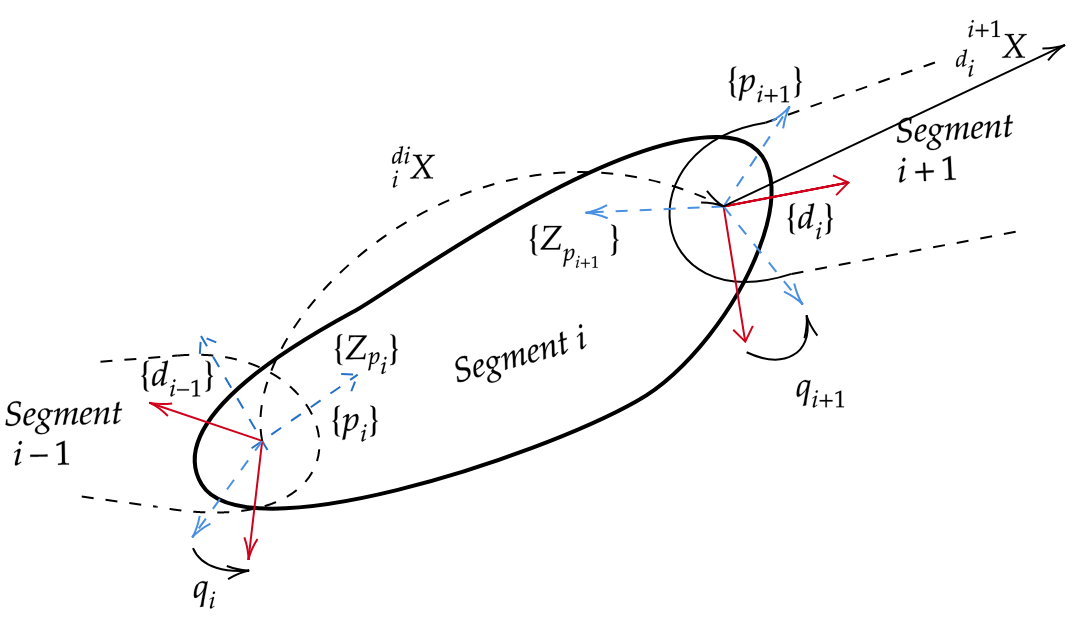
\includegraphics[scale=0.33]{images/pose.png}
	\caption{Proximal and distal segment frames attachment in a generic kinematic chain and transformation between them~\cite{shakhimardanov2015composable}.}

\end{figure}

In line \ref{4}, the \textit{spatial velocity vector} of segment $i+1$ is calculated, which is represented by $\ddot{X}_{i+1}$. The expression is evaluated as the summation of $\prescript{i+1}{}{X}_i\ddot{X}_i$ and  $S_{i+1}\dot{q}_{i+1}$ recursively. Here the first term represents velocity of segment $i$ expressed in the coordinates of segment $i+1$. The transformation from link $i$ to $i+1$ is computed by matrix $\prescript{i+1}{}{X}_{i}$. The second term refers to joint velocity contributions ($\dot{q}_{i+1}$) that is expressed using motion subspace matrix ($S_{i+1}$).

	The next equation (line \ref{5}) denotes \textit{bias acceleration} at segment $i+1$, noted as $\ddot{X}_{bias, i+1}$. Since the joint acceleration components are unknown at this stage, only the bias acceleration is computed, provided the Cartesian and joint space acceleration of previous link. Here, $\dot{X} \times S \dot{q}$ acts as time derivative of $S$, that maps from velocity to acceleration domain. 
% The cross product denotes the cartesian space acceleration expressed in link coordinates and 

Furthermore, \textit{bias forces} are determined by the expression in line \ref{6}, given the Cartesian velocity vector, $\dot{X}_{i+1}$ and inertia matrix, $H_{i+1}$. The term $\times^*$ is the cross product operator expressed in Pl{\"u}cker coordinates (refer to appendix section \ref{chap:cross} for explanation on spatial cross products). The bias forces is influenced by the \textit{external forces} as well, given by $F^{ext}_{0, i+1}$ and is transformed from base to end-effector coordinates, expressed by transformation matrix for force vectors, $\prescript{i+1}{}{X}_0^*$. See the appendix section \ref{chap:coordinate} for coordinate transformation on force and motion vectors.

In the line \ref{7} and \ref{8}, \textit{articulated body inertia} and \textit{articulated bias forces} respectively are initialized with \textit{rigid body} quantities. These values are further used in inward sweep.

\subsection{Inward sweep : force and inertia recursions} \label{inward-sweep}

A set of recursive equations in inward sweep computes force and inertial parameters of every segment. The joint torques and external forces acting on the distal segments collectively generates \textit{inertia-dependent acceleration} on the proximal segments~\cite{shakhimardanov2015composable}.


In line \ref{11}, the combined inertias of segment $i+1$ and joint rotor inertia ($d_{i+1}$) is computed. Matrix $P_{i+1}$ is a projection matrix, that projects \textit{articulated body inertia} and \textit{bias forces} over joint subspace~\cite{shakhimardanov2015composable}~\cite{vukcevic2018extending}. In further steps, the algorithm calculates \textit{apparent inertia} (line \ref{13}) represented as $H^a_{i+1}$, which is the inertia contributions from the child segments. And \textit{articulated body inertia} (line \ref{14}) denoted as $H^A_{i}$ is calculated by adding all the apparent inertias. Similarly, apparent ($F^a_{bias, i+1}$) and articulated bias forces ($F^A_{bias, i}$) are computed by expression in line \ref{15} and \ref{16} respectively.

In expression \ref{17}, \textit{constraint force matrix} is computed ($A_i$), in which the term $P_{i+1} A_{i+1}$, represents apparent unit constraint forces. Consequently, these constraint forces, external forces and joint torques inclusively generates acceleration energy~\cite{shakhimardanov2015composable}, which is recursively accumulated in matrix $U_i$ (line \ref{18}). Here, $U_i$ is \textit{acceleration energy} matrix expressed in Cartesian space. The expression within curly braces denotes acceleration originated from joint torques, and inertial forces applied at distal joints~\cite{shakhimardanov2015composable}.

The inward recursion also deals with constraint acceleration energy, $b_N$, that is produced by corresponding columns of constraint forces, $A_N$~\cite{shakhimardanov2015composable}. This is represented by $\mathcal{L}_i$ (line \ref{19}) and is called \textit{constraint coupling matrix}, which is of order $m \times m$ ($m$ is number of constraints). More clearly, each rows in $\mathcal{L}_i$ corresponds to acceleration energy generated by all the constraint forces and accelerations, up until that instance of recursion.

\begin{figure}[h!]
	\label{fig:sweep}
	\centering
	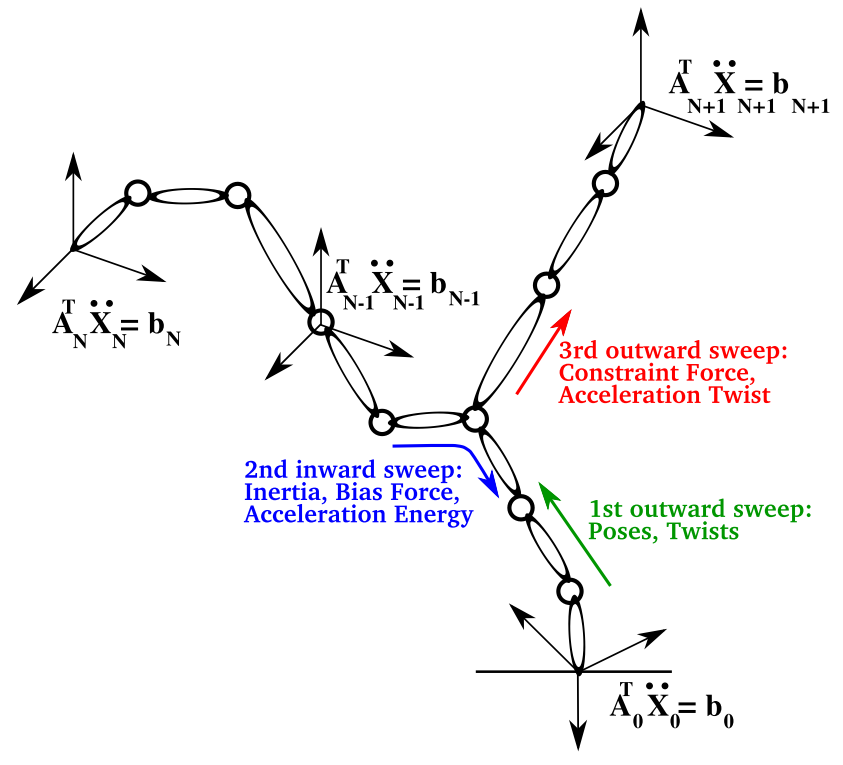
\includegraphics[scale=0.35]{images/sweep.png}
	\caption{An abstract representation of computational sweeps in a kinematic chain, along with computed physical entities and constraints (source:~\cite{shakhimardanov2015composable})}.	
\end{figure}

\subsection{Computing constraint force magnitudes, $\nu$}

After reaching the base ($i = 0$), the \textit{constraint force magnitudes} are calculated (line \ref{21}). This expression is obtained after minimizing the Equation \ref{eq:bellman} with respect to $\nu$~\cite{shakhimardanov2015composable}. The constraint force magnitude is a scaling factor that is computed by ratio of generated acceleration energy ($\mathcal{L}_0$) to required acceleration energy, ($b_N -  A_0^T \ddot{X}_0 - U_0 $). The term $\ddot{X}_0$ denotes the Cartesian acceleration at the base. Since the base is rigidly fixed in a kinematic chain, $\ddot{X}_0$ is equal to acceleration due to gravity. 

It is however important to ensure that the matrix $\mathcal{L}_i$ is of full rank. But this case fails during singularity. To overcome this situation, ($\mathcal{L}^{-1}$) can be computed using the \textit{damped least squares} method, as mentioned in~\cite{shakhimardanov2015composable}.

\subsection{Outward sweep : Control torques and link accelerations}
In the outward sweep, the control torques and joint accelerations of the constrained motion are computed (line \ref{23} and \ref{24})~\cite{shakhimardanov2015composable}. After minimizing the equation \ref{eq:bellman} with respect to $\nu$ in previous step, the \textit{constraint force magnitudes} is substituted and solved for joint acceleration $\ddot{q}_i$ in the final outward sweep. As mentioned before, the joint $i+1$ experiences external and Coriolis forces ($F_{bias, i+1}^A$), inertial forces ($H_{i+1}^A\prescript{i+1}{}{X}_i \ddot{X}_i$) and feed-forward torques ($\tau_{i+1}$) from the connected child segments. Corresponding to these quantities, the equation in curly braces (line \ref{23}) represents the overall control torque that is required to drive the constrained system~\cite{vukcevic2018extending}.

Reformulating the expression in line \ref{23} and representing the torque components as (see equation \ref{eq:jointaccl})~\cite{vukcevic2018extending},
\begin{equation}\label{eq:jointaccl}
	\ddot{q}_{i+1} = D_{i+1}^{-1} \big\{ \overbrace{\strut \tau_{i+1}}^\text{input torque} - \underbrace{ \strut S_{i+1}^T \big(F_{bias, i+1}^A + H_{i+1}^A \big(\prescript{i+1}{}{X}_i \ddot{X}_i + \ddot{X}_{bias, i+1}))}_\text{bias torque} - \overbrace{\strut S_{i+1}^T A_{i+1} \nu}^\text{constraint torque} \big \}
\end{equation}

In the final step of the algorithm, spatial acceleration $\ddot{X}$ is computed (line \ref{24}) by substituting $\ddot{q}$ from the previous step. 

Figure \ref{fig:sweep} describes the computational sweeps in a kinematic chain.


\section{Task Specification}

The Popov-Vereshchagin Hybrid Dynamic solver computes the desired motion of manipulator accounting to the task specification. The inputs to the solver includes three kinds of task definitions - \textit{External force}, \textit{Cartesian acceleration constraints} and \textit{feedforward torque}. This section further explains these task definitions.

\begin{enumerate}
	\item \textit{\textbf{External forces} ($F_{ext}$):} \\
	The external forces (physical or virtual) applied to the end-effector can be used for \textit{impedance control} in Cartesian space~\cite{siciliano2016springer}. The resulting impedance control is required to ensure a compliant behavior of end-effector~\cite{albu2002cartesian}. 
	
	\item \textit{\textbf{Cartesian acceleration constraints:}} \\
	The task requirements imposes \textit{Cartesian acceleration constraints} on manipulator motions. There are two distinct types of constraints that can be applied on the segments - \textit{physical} and \textit{virtual}. The former refers to environmental contacts, whereas the latter defines the desired Cartesian accelerations as specified by the user~\cite{shakhimardanov2015composable}. 
	
	Consider a manipulator with $N$ segments. The \textit{virtual} constraints are specified in matrix $A_N$ of order $6 \times m$, where $m$ is number of constraints. The columns of the matrix represent direction of constraint forces being applied on end-effector. As mentioned in section \ref{inward-sweep}, the acceleration constraints produces \textit{acceleration energy}, represented by $b_N$. The expression for linear constraints is given in equation~\ref{eq:constraint1}. For instance, if the user defines partial constraints to restrict the motion of a segment in $x$ and $z$ directions linearly, then the $A_N$ matrix can be written as follows,
	\begin{equation}\label{eq:A}
	A_N = 	\begin{bmatrix}
	0 & 0 \\
	0 & 0 \\
	0 & 0 \\
	1 & 0 \\
	0 & 0 \\
	0 & 1 \\
	\end{bmatrix} 	
	\end{equation}
	
	As the motion is restricted, the accelerations should be $0$ in $x$ and $z$ directions. The acceleration energy vector can be specified as, 
	
	\begin{equation} \label{eq:bN}
	b_N = \begin{bmatrix}
	0 \\ 
	0 \\
	\end{bmatrix}
	\end{equation}
	
	Similarly, acceleration constraints can be defined in all six dimensions. Correspondingly, the acceleration energy vector must be specified. 
	
	\item \textit{\textbf{Feedforward torque ($\tau$):}} The input torque is equivalent to joint constraints. This can be used in tasks that require posture control. For instance, in case of manipulators, to remain in a vertical orientation, the joints are provided with feedforward torques~\cite{sentis2005synthesis}.
	
	\end{enumerate}
	
	In case of a high level task specification, all the three types of task definitions (as explained previous section) are provided as input to the robot controller. The general control scheme including the solver is presented in~\cite{vukcevic2018extending} as,
	
	\begin{figure}[h!]
		\label{fig:control-scheme-solver}
		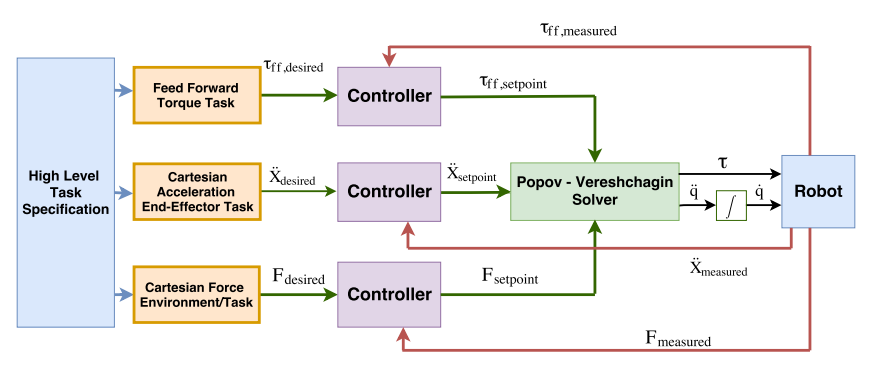
\includegraphics[scale=0.5]{images/control-scheme-solver.png}
		\caption{General control scheme including the Vereshchagin solver (source:~\cite{vukcevic2018extending})}
	\end{figure}

\section{Solver Implementation}

The Vereshchagin solver is currently implemented using Kinematics and Dynamics library~\cite{KDLopensource}, by Herman Bruyninckx, Azamat Shakhimardanov and Ruben Smits. The library is an \textit{open source} and the solver is currently built in C++ programming language. 



%\section{Modeling kinematic tree for Care-O-Bot}{......}

